\documentclass{article}


\usepackage{arxiv}

\usepackage[utf8]{inputenc} % allow utf-8 input
\usepackage[T1]{fontenc}    % use 8-bit T1 fonts
\usepackage{hyperref}       % hyperlinks
\usepackage{url}            % simple URL typesetting
\usepackage{booktabs}       % professional-quality tables
\usepackage{amsfonts}       % blackboard math symbols
\usepackage{nicefrac}       % compact symbols for 1/2, etc.
\usepackage{microtype}      % microtypography
\usepackage{lipsum}
\usepackage{graphicx}
\graphicspath{ {./images/} }


\title{Embedded and Distributed AI - Real Time SLAM Project Report}


\author{
 Jonatan Flyckt \\
  School of Engineering\\
  Jönköping University\\
  Gjuterigatan 5, 553 18 Jönköping \\
  \texttt{fljo1589@student.ju.se} \\
   \And
 Marcus Gullstrand \\
  School of Engineering\\
  Jönköping University\\
  Gjuterigatan 5, 553 18 Jönköping \\
  \texttt{guma1502@student.ju.se} \\
}

\begin{document}
\maketitle
\begin{abstract}

Simultaneous localisation and mapping (SLAM) can be used to create maps of areas while simultaneously detecting and mapping an agent's position in these maps through the use of various sensors. The objective of our project was to create an intuitive and easy-to-use SLAM implementation using mainly the camera sensor on mobile Android devices that could show accurate 2D floor-plan style maps. By using Google's ARCore library to extract SLAM landmarks, we created an application that continuously plots and updates a 2D map using the Android Canvas library. The resulting application works well in well-lit indoor areas, as well as outdoor areas without inclination. However, the application perform poorly when there is a lot of incline, or when the scanning area is too dark to accurately detect landmarks. Our application has room for improvements with regards to processing performance, better landmark collection, and more accurate plotting. Although the application has issues, the final result is a fun and intuitive application that can be used by anyone with a mobile Android device.

\end{abstract}

\section{Introduction}
\subsection{Background}

SLAM is the technique of continuously and incrementally building a map of an environment, while also simultaneously localising the position of some agent (often a mobile robot) in this environment \cite{background1}. The SLAM problem is of great interest to the robotics community, and SLAM is used by both indoor and outdoor robots, as well as in underwater and airborn systems \cite{background1}. In recent years, SLAM has also seen successful use in commercial semi-autonomous vehicles such as Tesla cars \cite{autonomous-cars}. The process of SLAM involves the agent moving through the environment and using one or more sensors to calculate an unknown number of landmarks by observing their relative position between different time frames \cite{background1}. Common sensors for SLAM are cameras, Sonars, and Lasers \cite{background2}.

\autoref{fig:slam} shows a simple SLAM scenario of a robot moving through an environment, estimating its position as well as the positions of discovered landmarks. At a time instant $k$, there are several different data gathered. $\textbf{x}_k$ shows the location and orientation of the robot. $\textbf{u}_k$ shows the applied state change at time $k-1$ to move the robot to its $\textbf{x}_k$ state. $\textbf{m}_i$ denotes the estimated location of the observed landmarks. $\textbf{z}_{ik}$ is the observation of the landmark $i$ at the time $k$. These data quantities constitute the essence of a SLAM algorithm. \cite{background1}

For all times $k$, a joint posterior density probability distribution needs to be calculated to determine how accurate the mapping of an $\textbf{m}_i$ landmark and the state $\textbf{x}_k$ of the vehicle is. This is calculated using Bayes theorem recursively with the following formula: $P(\textbf{x}_{k-1}, \textbf{m} | \textbf{Z}_{0:k-1}, \textbf{U}_{0:k-1})$. A map $m$ of all landmarks can then be constructed by combining the landmarks of all the observations from different locations. \cite{background1}

Visual-Inertial SLAM (VISLAM) is a SLAM method that uses a visual sensor (camera) as well as on-board edge sensors such as gyroscope and accelerometer to accurately detect the gravitational direction, producing correct axes relative to earth. VISLAM is also generally a cheaper alternative to laser-based approaches. \cite{vislam}


\begin{figure}[!htb]
    \centering
    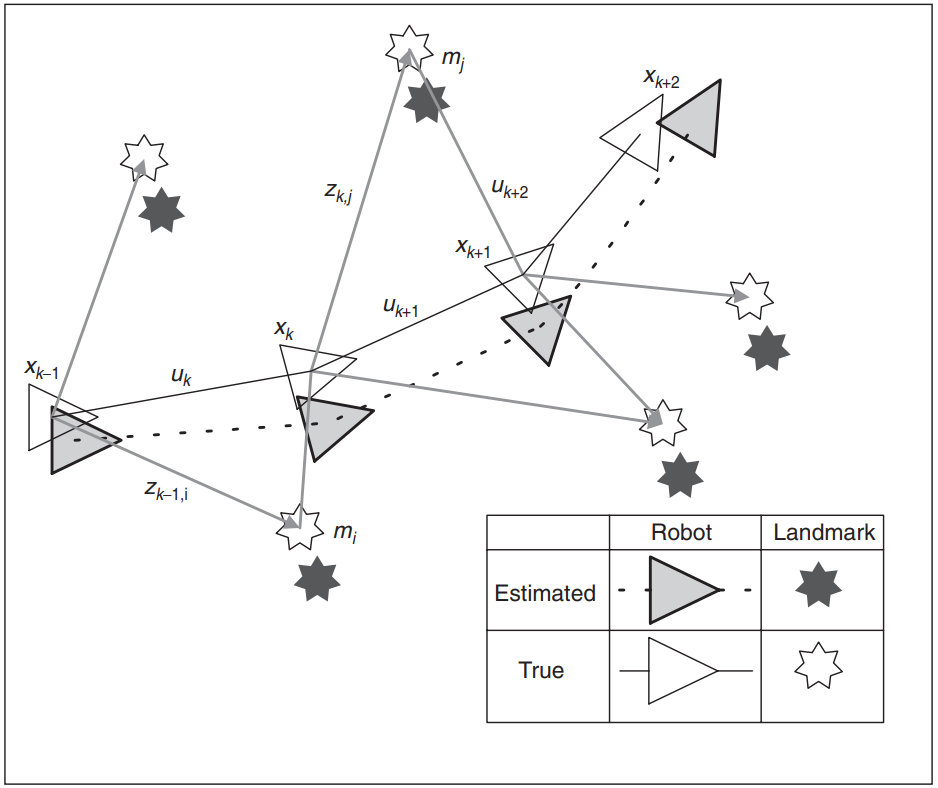
\includegraphics[width=0.6\linewidth]{slam.PNG}
    \caption{The SLAM problem. A robot moving through an environment and observing landmarks, estimating its own, and the landmarks' locations. Source: \cite{background1}}
    \label{fig:slam}
\end{figure}
% Introducera SLAM som koncept. Vilken kombination av teknologier används för att möjliggöra SLAM generellt sett? Vilka typ av sensorer kan användas i olika tillämpningar (LiDAR etc)? 'Man behöver en kamera... etc.'

\subsection{Problem description}
In this project, we attempt to use the VISLAM implementation of Google's ARCore library \cite{ARCore} to map spatial environments on mobile Android devices. Mobile Android devices were chosen for several reasons:
\begin{itemize}
    \item They are user friendly and intuitive.
    \item They are mobile and easy to move around with in any environment.
    \item Phones and other Android devices have built-in sensors in addition to camera (such as accelerometers and gyroscopes), which help in producing accurate maps of the real world with the earth as a reference point. This is often not possible when for example using solely a camera on a laptop or some other device.
\end{itemize}

The focus of the project is to build a user-friendly Android mobile application that produces an accurate mapping of the environment, and the device's position in that environment. We display both a live camera feed with landmarks overlayed in real-time, as well as a map plot where the landmarks have different colours based on the confidence with which the SLAM has estimated their positions. This should help the user to understand the SLAM process intuitively, and aid in the gathering of better landmark points, and in extension a better overall mapping of the spatial environment.

Because we could not find any free-to-use open source 3D plotting libraries for Android, we elected to instead plot the map and localisation in 2D with a from-above view. This meant that we had to do extensive calculations on the 3D landmark points to accurately represent the environment in a floor-plan style.


% Vad vill vi göra med SLAM? (Vi vill anskaffa oss en 2D karta över området där SLAM påbörjas som inkluderar ens egna position). Varför valde vi mobil? Vi ville ha en användarvänlig SLAM-upplevelse.

\section{Method}
\subsection{ARCore}
%Motivera varför vi valde google ARCore. Berätta hur ARCore fungerar (nämn gyro och accelerometer), vilken SLAM-metod använder ARCore, och hur räknas confidence ut?

%https://developer.android.com/guide/topics/sensors/sensors_motion
%Motion Tracking (Concurrent odomentry & Mapping)

%https://developers.google.com/ar/discover/concepts
%ARCore

ARCore consists of 3 parts: 'Motion tracking', 'Enviromental understanding' and 'Light estimation'. In this project we only used motion tracking, which esentially is SLAM. The latter two parts has to do with placing 3D objects on surfaces (e.g. a table, the floor etc.) and giving them the appropriate amount of lighting or shading depending on the given lighting conditions. We excluded these two parts from the sample project that we used. \cite{ARCore}

Motion tracking in ARCore is the combination of processed visual information (Computer vision) and spacial information about the device from inertial measurements (accelerometer data, gyroscope data, rotation etc.). The visual information, given as at least two or more feature points in an image frame, and information about the phone relative to the earth gives the combined information of points of interest in each image frame that have the correct orientation and position relative to the phone and to the earth. \cite{ARCore}

For each point of interest in each image frame, ARCore calculates a confidence that indicates how sure it is that that point is representing an accurate description of reality. The confidence is on a scale of 0 to 1, 0 being not sure at all and 1 being so sure that it is essentially a fact. We could not find any documentation of how this confidence calculation is performed. However, the confidence values showed very good results, so we still use them in our application when deciding which landmarks to add, as well as what landmarks to prune from the map.

\subsection{Landmark processing} \label{landmark-processing}
%Berätta hur vi hämtar ut landmarks och processerar dem. Berätta hur vi målar ut allt på skärmen.

The landmarks are extracted from the SLAM algorithm's stream of landmarks that are currently in view by the camera sensor. Each landmark contains 4 variables:
\begin{itemize}
    \item X position in metre distance from camera origin (left and right relative to phone's starting position)
    \item Y position in metre distance from camera origin (forward and back relative to phone's starting position)
    \item Z position in metre distance from camera origin (up and down relative to the earth)
    \item Confidence level
\end{itemize}
Because the landmark stream updates several times per second, and can contain very many landmarks at any one time (many hundreds), several pruning measures need to be taken when deciding which landmarks to keep and visualise. Every time a set of landmarks are extracted from the stream, they are run through a set of post-processing steps, and either removed permanently, or stored and drawn on the map.

We use the calculated confidence of each landmark to decide whether it should be pruned or kept. However, if we used the overall confidence of all landmarks and only kept the ones with the best confidence, the map would only contain points that lie in positions that are easy to map well, removing points in hard to scan areas completely. To circumvent this problem, we divided the map into a set of grids of $0.25 * 0.25$ m, each with its own set of up to 300 landmarks. These landmarks were pruned per individual grid zone, meaning that poorly scanned areas would never be removed, but only updated if that same area was scanned again. This meant that for each $m^2$ of scanned landmark points, there exists 16 grid zones and a total of up to 4800 landmark points.

The landmarks are pruned roughly once per second. To save processing power, it is kept track of which grid zones have received new landmarks since the last pruning, and only updated zones are pruned. In addition to pruning the grid zones based on confidence, we also prune and completely remove grid zones with very few landmarks (fewer than 40). This is done to prevent incorrect outliers to be stored and displayed to the user. Another measure taken to prevent outliers is that only landmarks with a confidence of at least 0.5 are saved. We also noticed early on that sometimes landmarks that were up to 40 meters away from the scanned area could be added erronously (for instance when looking through the window of an apartment). Therefore, we only save landmarks if they are within 1.5 metres of an existing previous landmark.

After pruning the newly added landmarks, all landmarks are iterated over to try to estimate the position of the floor in the spatial environment. We do this by identifying what Z axis interval of 0.25 metres (below the average camera position) that contains the most points. This is done to make the visualisation of landmarks to the user better, and will be explained more thoroughly in the \nameref{landmark-visualisation} section. The step-by-step process of landmark pruning is described in the \nameref{workflow} section.

\subsection{Landmark and localisation visualisation} \label{landmark-visualisation}
The landmarks and phone position are visualised as a 2D map in a view below the camera view in the application. Several possible visualisation libraries (both 2D and 3D) were examined before settling on manually drawing the map every frame with the Android standard Canvas library, as this granted us the most control over what to show the user. Each landmark is drawn as a small dot on the canvas, and the position of the phone throughout a SLAM session is stored as a line showing the movement of the phone, and the current phone position as a large dot. The canvas is redrawn 20 times per second, to make the application feel fluid. This, however, means that as more landmarks are scanned, the application is quite draining for the phone's performance; a fully scanned environment of 50 $m^2$ contains 240 000 individual points. Each landmark dot is visualised on a scale from red to green, where red indicates a low confidence, and green indicates a high confidence. This is done to intuitively show the user what areas need to be scanned again.

Because the scanned area can grow continuously throughout a SLAM session, the view needs to be zoomed out as more areas are discovered. This zoom is designed to feel fluid to the user. The scale in which to display the landmarks is calculated by looking at the pixel size of the view and the extreme x and y points that have been scanned. Because landmark positions can have negative values, and are expressed as float point values as metres from the original camera position. The pixel points at which to display each single landmark needs to be recalculated for each screen update.

To show the user an accurate 2D representation, we also need to exclude points scanned close to the floor. If this was not done, the mapping would look like a mess of points all over the map. To accomplish this, we calculate the average Z axis position of the phone (usually at roughly 1.5 metres height) as well as the estimated floor position (as described in the \nameref{landmark-processing} section). The alpha of each point is then continuously lower the closer to the floor the point is (with an alpha of 0 at the floor).

\autoref{fig:scan-example} shows the application design and results from detailed scans of two separate well-lit indoor areas.

\begin{figure}[!htb]
    \centering
    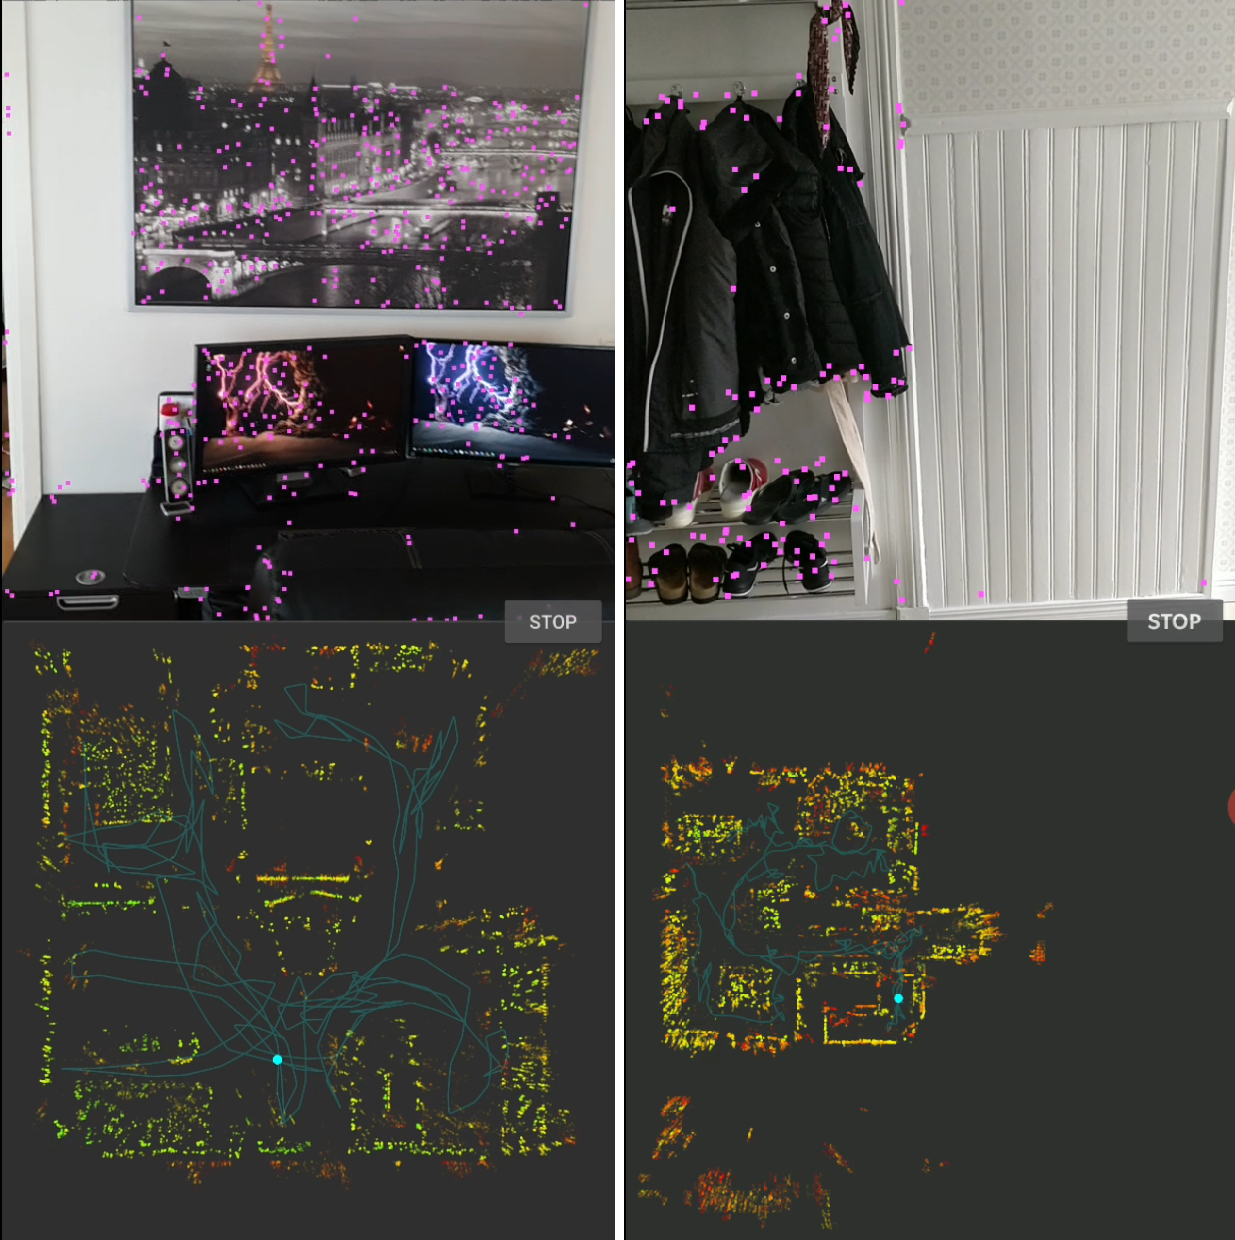
\includegraphics[width=0.6\linewidth]{scan-example.png}
    \caption{Screen grabs from two detailed scans of well-lit indoor areas. The results are accurate floor-plan maps where floor landmarks are excluded.}
    \label{fig:scan-example}
\end{figure}

\newpage
\subsection{Workflow} \label{workflow}
\autoref{fig:workflow} shows a workflow of the running application for each landmark update iteration.
\begin{figure}[!htb]
    \centering
    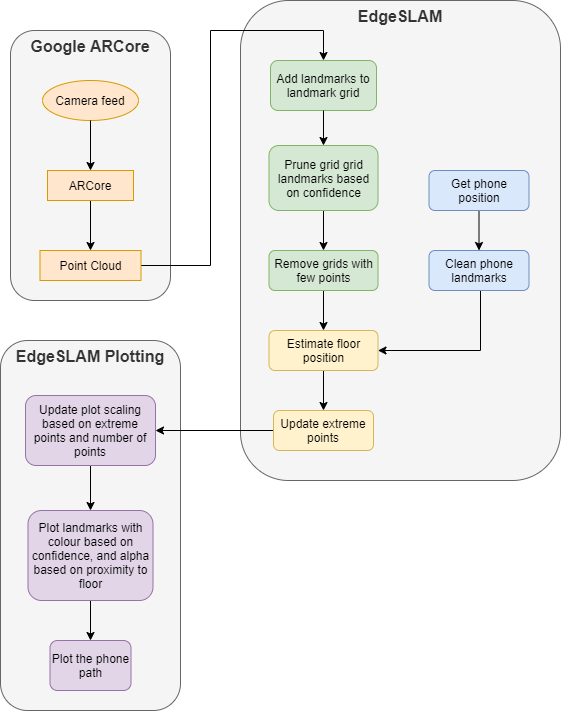
\includegraphics[width=0.9\linewidth]{EdgeSLAM Workflow Diagran.png}
    \caption{Workflow describing the SLAM and visualisation measures taken by our application at each iteration of landmark updates (roughly once per second depending on device).}
    \label{fig:workflow}
\end{figure}

\clearpage
%\subsection{Our implementation in conjunction with ARCore}
% Varför målar vi ut på detta sättet? Varför 2D? Workflow-diagram som förklarar från sensorinsamling till utmålning.
% Varför 2D och inte 3D? Svårigheter?

\section{Discussion and Results}
\subsection{Strengths and weaknesses}
%Diskutera svagheter och styrkor med vår metod. Visa bilder och diskutera specifika scenarier och hur appen reagerar på dem.

The overall performance of the SLAM is good when the scanning conditions are sufficient (good lighting and not a lot of dark zones). However, if the area that is being scanned is too dark, the camera will be unable to accurately make out feature points (\autoref{fig:dark-no-landmarks}, \autoref{fig:good-poor-scan}). Lack of lighting is a general problem in visual-based SLAM methods \cite{dark}. The application runs smoothly on most devices. However, when the amount of scanned points reaches a certain level, the application starts to run slower on devices with a worse CPU.

\begin{figure}[!htb]
    \centering
    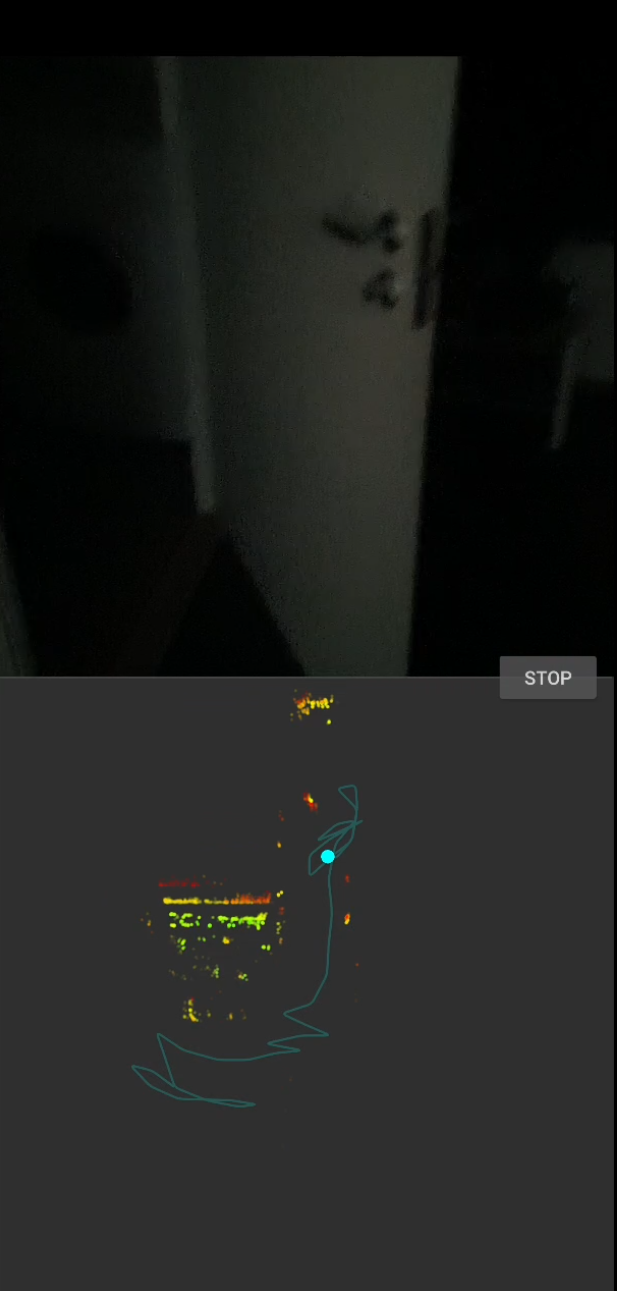
\includegraphics[width=0.2\linewidth]{dark-no-landmarks.png}
    \caption{In dark areas, the SLAM does not manage to detect any single landmark.}
    \label{fig:dark-no-landmarks}
\end{figure}

\begin{figure}[!htb]
    \centering
    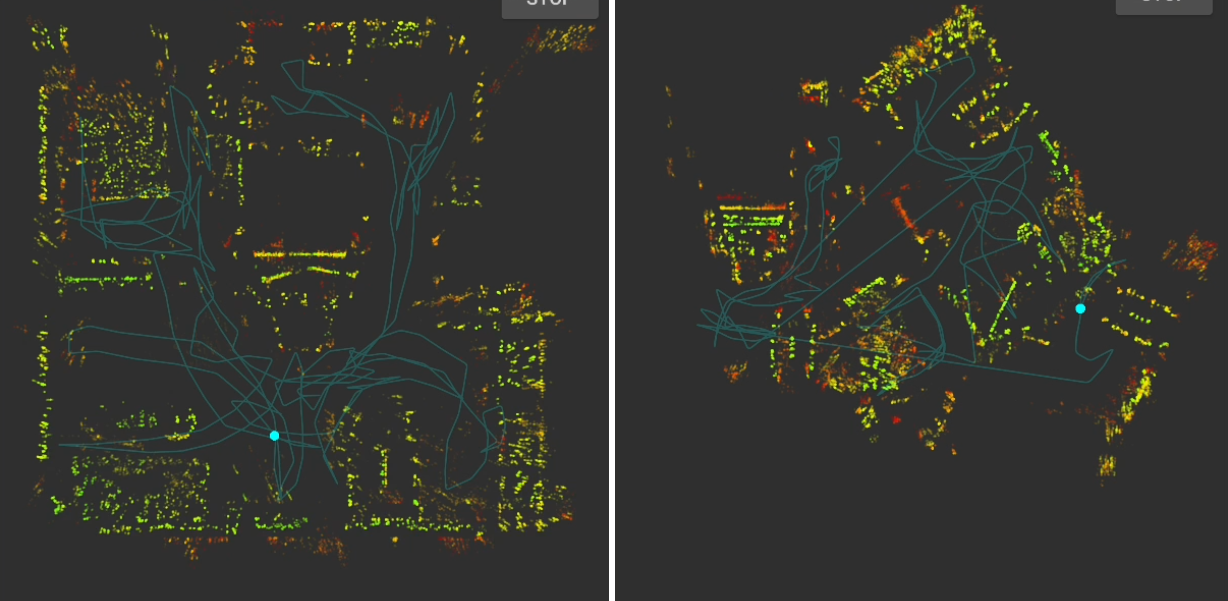
\includegraphics[width=0.8\linewidth]{good-poor-scan.png}
    \caption{The difference between sufficient and insufficient lighting. The same area has been scanned, but the picture on the right has had poor lighting conditions, whereas the picture on the left has had excellent lighting conditions. The SLAM on the right has lost track of its position several times and plotted in incorrect areas. It is also clear that a lot fewer landmarks (and with worse confidence) have been picked up.}
    \label{fig:good-poor-scan}
\end{figure}

The application is very good at picking up landmark points and mapping them accurately when there are a lot of unique reference points. For instance: paintings, kitchen tiles, blankets, pillows, couches etc. all yield very good landmark points. The application is also very good at showing to the user what is being scanned in the camera overlay, as well as in the real-time plot update. Like all visual based SLAMs, the performance is much worse when the scanned area is "blank", i.e. it does not contain a lot of texture or colour differences. An example is a white ceiling or a white wall, which will be poorly mapped by the SLAM algorithm.

Our application is tuned mainly to be used in flat areas, as floor level landmarks need to be excluded to produce a good map in a 2D view. This means that scanning areas with a lot of incline sometimes can produce weird results. Because we reduce the alpha of points at an estimated floor level, incorrect reduction of alpha values can occur. This can be clearly seen in \autoref{fig:floor-recalibration}, where the severe incline of the garden being scanned causes the floor estimation to "jump" as more areas are scanned. 

\begin{figure}[!htb]
    \centering
    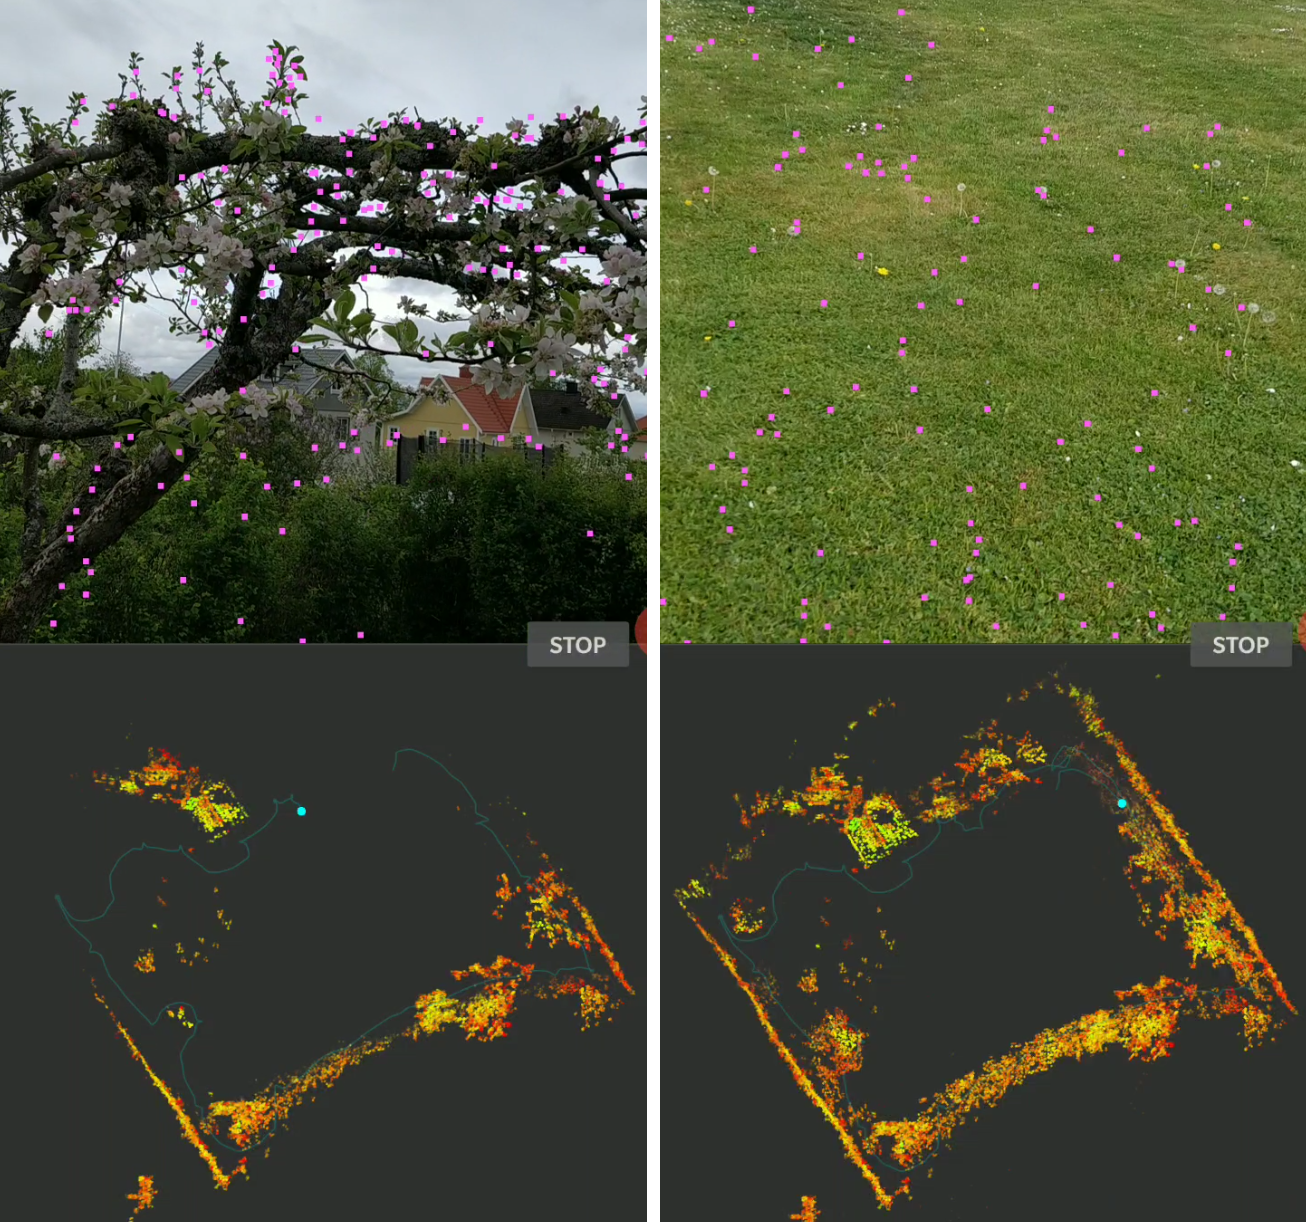
\includegraphics[width=0.6\textwidth]{floor-recalibration.png}
    \caption{The effects of floor position estimation. In an area with a lot of incline, the floor position is continuously re-estimated, producing incorrect maps a lot of the time.}
    \label{fig:floor-recalibration}
\end{figure}

Although measures were taken to exclude outlier points scanned through windows (only points with good confidence within 1.5 metres of previously scanned areas were added), sometimes the application included outdoor points. This generally occurred when the outdoor points were on the same height as the indoor points (meaning that the points were close enough to be included) (\autoref{fig:mirror-window-examples}). Another problem with our application is that looking through mirrors caused the application to perceive the reflection as an entirely separate room. This can be seen in \autoref{fig:mirror-window-examples}. If the slam had been laser or sonar based, these landmarks would never be created, but we have no good suggestion for how to remove these inaccuracies with a camera-based SLAM method.

\begin{figure}[!htb]
    \centering
    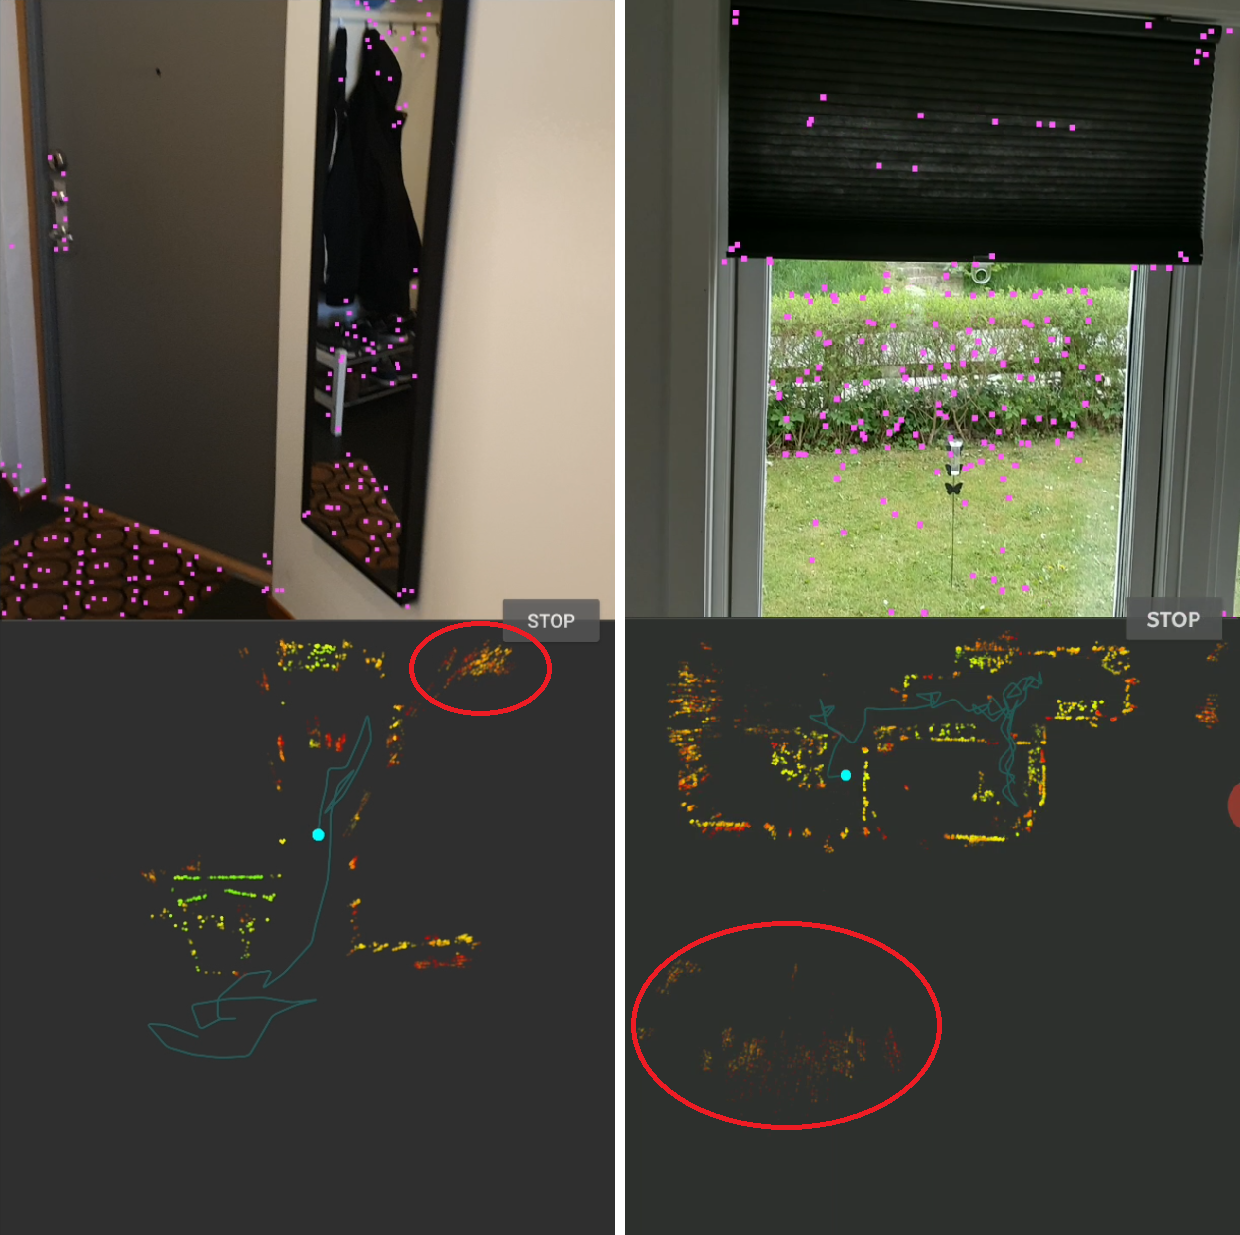
\includegraphics[width=0.6\linewidth]{mirror-window-examples.png}
    \caption{The left image shows the SLAM inaccurately detecting mirror reflections as a separate new room. The right image shows the SLAM detecting and plotting outdoor points.}
    \label{fig:mirror-window-examples}
\end{figure}

Due to time limitations, we spent limited time on examining the features of the ARCore library. ARCore performs loop closing (adjusts all landmark positions after reaching an area previously scanned), but this will not work perfectly on our application because we extract and save the landmarks in our own structure. We also have no control over the computer vision measures that ARCore takes to extract the landmarks, but have to rely on the algorithm extracting the landmark points. ARCore also contains limited documentation as to how this is done, so it is hard to analyse how, and if, it could be done better.
%Ta intressanta fakta från videor.

%Vad funkar bra?
% appen på en bra device
% hitta punkter som inte är golv/tak
% Ju längre man scannar desto bättre blir en punkt (och appen är bra på att visa det för användaren)



%Vad funkar dåligt?
% Plana ytor utan textur blir dåliga
% Vi sparar alla landmarks själva.
% "Ingen" loopclosing
% Inte kontroll över computer vision algoritmen (ARCore är som en blackbox i hur den får ut sina intresse-punkter)

\newpage
\subsection{Conclusions and future work}
Our application is fun and can be used to receive an accurate mapping of most well-lit areas, both indoor and outdoor. It is intuitive to use with points in different colours showing what areas are scanned well or not. The application also produces good 2D floor-plan maps by excluding floor points. However, it maps poorly in areas with a lot of incline. For it to be useful as an instantaneous mapping for an automated vehicle or similar, the app would need to be optimised a bit more. Future work could include making the app more friendly to devices with poor hardware. We could also make use of ARCore's built-in loop closing instead of manually extracting all landmarks and processing them separately. To circumvent issues with dark areas, we could also make use of the phone's LED lighting automatically when dark areas are reached. This was done by \cite{dark} with good results.
% Är det användbart i slutändan? Kan VÅRT arbete användas i ett verkligt scenario?

\newpage
\bibliographystyle{unsrt}  
\bibliography{references.bib}

\section*{Appendices}

\subsection*{Appendix 1: Application APK}

Use this link to download and install the application on an Android mobile device: \underline{\href{https://gofile.io/d/qrnUMs}{EdgeSLAM APK}}

\subsection*{Appendix 2: GitHub repository}

\underline{\href{https://github.com/jonatan-flyckt/edge-project}{Repository link}}

\textbf{GÖR EN CODE CLEAN MED KOMMENTARER OSV.}

Note: The application code is divided into two folders: "ARCore" and "EdgeSLAM". The code in the EdgeSLAM folder is produced by us (with the exception of some of the code in the SLAMActivity class), and all the code in the ARCore part is from the cloned ARCore repository.

\subsection*{Appendix 3: Video demonstration}
\underline{\href{https://www.youtube.com/watch?v=DzVZ3-SN9z8&feature=youtu.be&fbclid=IwAR3qJmJFWr76Q3OxECmys8Ir4qt6TEGevo86pbrAXv_0whPho_CLZh_HW-M}{YouTube video demonstrating our application running in live environments}}

\end{document}
